\chapter{Materials and Methods} \label{chap:materials}

\section{Genomic Data Preprocessing}

In this report, all genomic data was acquired from the National Cancer Institutes (NCI) genomic data portal \cite{grossman2016toward}. Healthy and tumorous cell mass RNA expresssion, microRNA expression, copy number variation, and simple nucleotide variation data was acquired for nine different forms of cancer and solid tissue normal (STN) samples. The nine cancer types included were head and neck squamous cell carcinoma (HNSC), kidney renal clear cell carcinoma (KIRC), kidney renal papillary (KIRP), liver hepatocellular carcinoma (LIHC), lung adenocarcinoma (LUAD), lung squamous cell carcinoma (LUSC), prostate adenocarcinoma (PRAD), thyroid carcinoma (THCA). The following subsections detail the preprocessing steps required to transform and extract features from the raw genomic data.

\subsection{Copy Number Variation}

\subsubsection{Preprocessing}

The copy number variation (CNV) data was derived from somatic and germline genotyping array (Affymetric Genome-Wide Human SNP Array 6.0). The raw CNV data is given as segmented genomic regions that have the same DNA copy number. This form provides the number of bound probes and the binary logarithm of the mean intensity (segmented mean) for each segmented genomic region as shown in Table \ref{table:rawcnv}.

\begin{table}[ht]
\caption{Raw CNV Data from Genome Wide SNP Segmentation} % title of Table
\centering % used for centering table
\resizebox{\textwidth}{!}{% % force table to text width
\begin{tabular}{l l l l l l} % centered columns (4 columns)
\hline %inserts single horizontal lines
GDC Aliquot $^a$ & Chr & Start & End & Probes & Segment Mean\\ %[0.5ex] % inserts table
%heading
\hline % inserts single horizontal line
% inserting body of the table
00e5b006-6afc-4ea4-90e3-f29741560020 & 1 & 62920 & 814954 & 31 & 0.4742\\
00e5b006-6afc-4ea4-90e3-f29741560020 & 1 & 817186 & 3303537 & 710 & -0.0539\\
00e5b006-6afc-4ea4-90e3-f29741560020 & 1 & 3303596 & 16477281 & 7873 & 0.0117\\
00e5b006-6afc-4ea4-90e3-f29741560020 & 1 & 16477846 & 16935737 & 127 & 0.3408\\
00e5b006-6afc-4ea4-90e3-f29741560020 & 1 & 16935752 & 30261189 & 7664 & 0.0229\\
% [1ex] adds vertical space
\hline %inserts single line
\end{tabular}}
\raggedright
\footnotesize{$^a$ Aliquot cooresponds to KIRC primary tumour UUID 0063a6fa-9ebd-4b71-83c0-aeb17b97eb6.}

\label{table:rawcnv}
\end{table}


\noindent
In order to extract features that can be shared between all nine cell mass types, the chromosomal regions were mapped to genes. Using the BioMart community portal we acquired the start and end positions of every gene in the human genome assembly GRCh38 (hg38) \cite{smedley2015biomart}. The human genes were then mapped to the CNV regions for each sample type. An example of the resulting process is shown in Table \ref{table:mapgene}.

\begin{table}[ht]
\caption{Significant CNV Abberations Mapped to Gene Ensembl ID in KIRC} % title of Table
\centering % used for centering table
\resizebox{\textwidth}{!}{%
\begin{tabular}{l l l l l l} % centered columns (4 columns)
\hline %inserts single horizontal lines
Ensembl ID & Chr & Abberration & Segment Mean & CNV Region & Gene Region\\ %[0.5ex] % inserts table
%heading
\hline % inserts single horizontal line
% inserting body of the table
ENSG00000237763 & 1 & DEL & -1.361 & 103620877-103717410 & 103655290-103664554\\
ENSG00000244057 & 1 & DEL & -1.9195 & 152583230-152613762 & 152600662-152601086\\
ENSG00000198502 & 6 & DUP & 1.9859 & 32488906-32533522 & 32517343-32530287 \\ 
ENSG00000264892  & 17 & DEL & -2.8409 & 16806233-16815664 & 16812447-16812651\\
ENSG00000279442 & 22 & DUP & 2.0311 & 15294547-15315221 & 15298378-15304556\\ 
% [1ex] adds vertical space
\hline %inserts single line
\end{tabular}}
\label{table:mapgene}
\end{table}

% GeneSymbol
% N/A
% AMY1A
% LCE3C
% HLA-DRB5
% NOS2P4
%Extra, just in case the Ensembl IDs dont fit
%TRGV4: ENSG00000211698 & 7 & DEL & -2.0425 & 38351764-38356875 & 38353715-38354517

\subsubsection{Dataset}

For the $i$-th cell mass, a set of $g_i$ genes were mapped to aberrant regions within the genome. The set of common genes between all cell mass types were defined as:

\begin{equation}
    \underset{i=1}{\overset{n}{\cap}} \; g_i,
\end{equation}

\noindent
Where $n$ is the number of cell mass samples. As a result, the CNV data contained the segmented mean of 11479 genes for each cell mass sample, resulting in a processed data matrix $C \in {\rm I\!R}^{11479 \; \times \; n}$.

\subsection{Transcriptome Expression}

\subsubsection{Preprocessing}

This study utilized RNA sequence (RNA-seq), and microRNA sequence (miRNA-seq) transcriptome expression profiling. The miRNA-seq data is a form of transcriptome profiling that provides miRNA molecule quantification. The miRNA-seq data used in this study was derived using the BCGSC miRNA profiling pipeline \cite{chu2015large}. Furthermore, RNA-seq is a form of transcriptome profiling that provides gene expression quantification. The RNA-seq data used in this study was derived from HTSeq-Counts framework \cite{anders2015htseq}.

All expression profiles were organized in relation to cancer subclass, individual case ID, and sequence ID. An example of this is shown in Fig. \ref{fig:expmirna}.

\begin{figure}[h!]
    \centering
    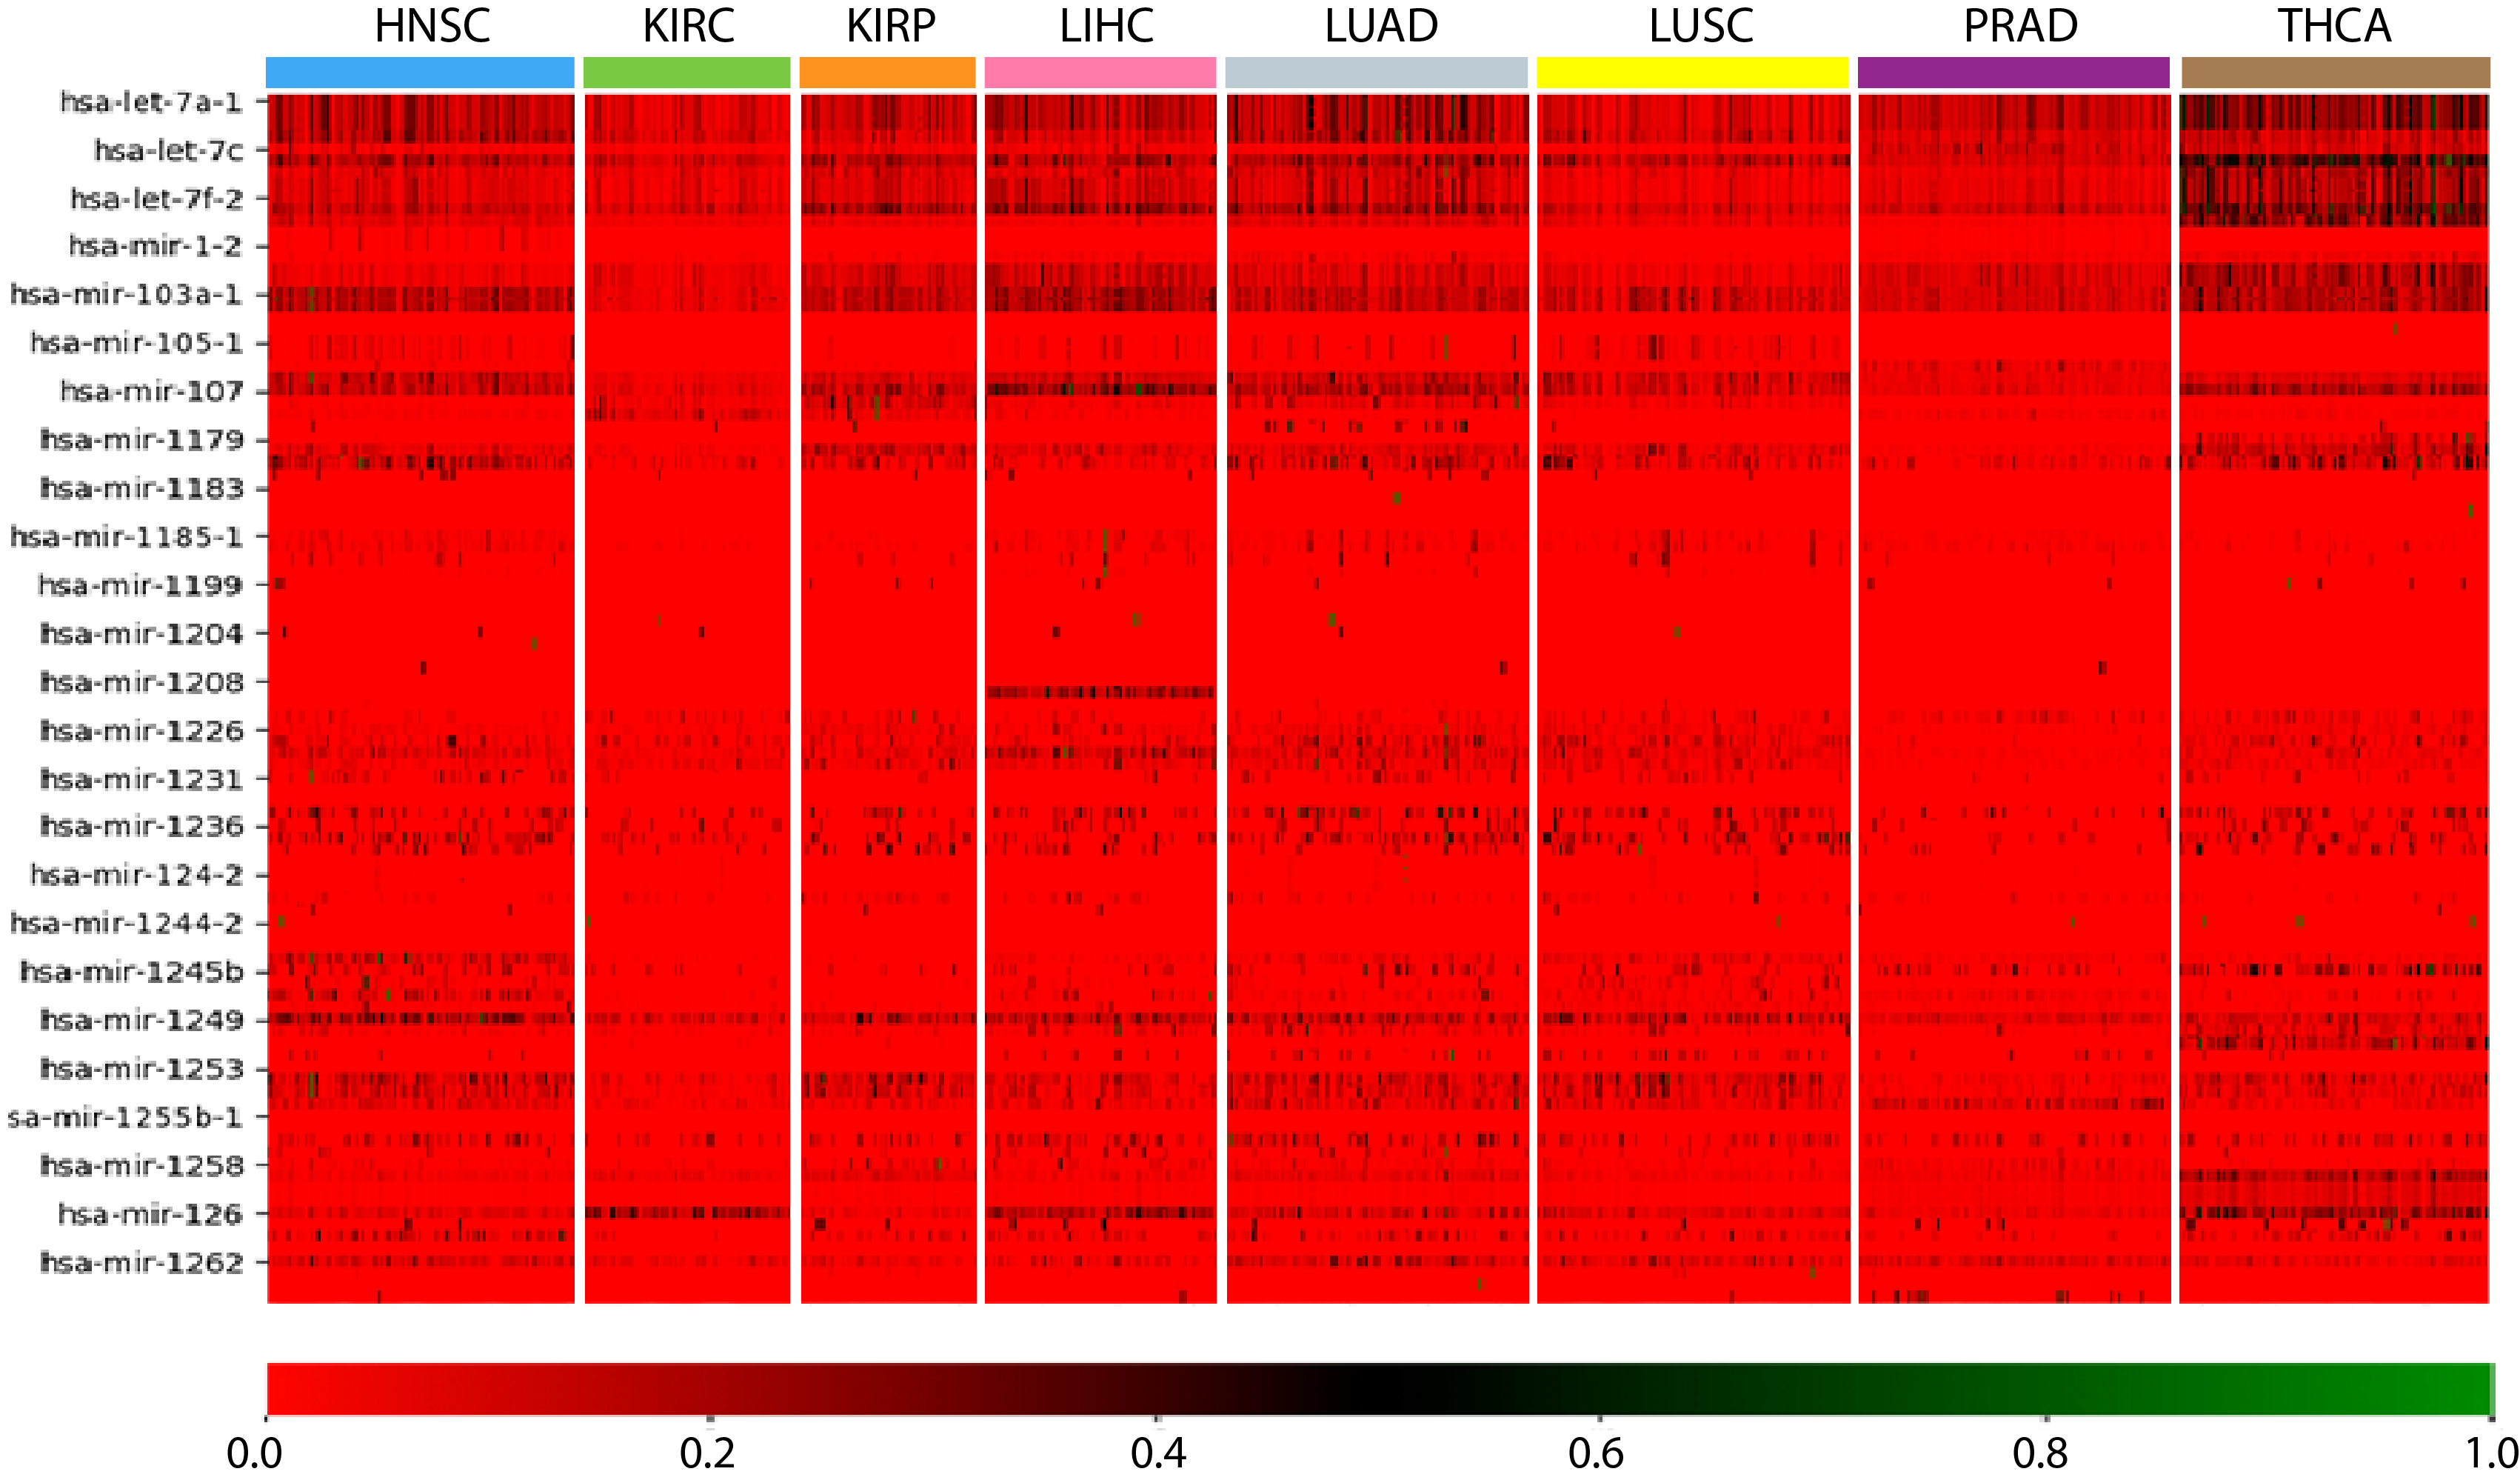
\includegraphics[width=\textwidth]{img/expmirna.png}
    \noindent
    \caption{Normalized miRNA expression profiles.}
    \label{fig:expmirna}
\end{figure}

\subsubsection{Dataset}

The expression profiles of the transcriptome expression data had the input feature dimensionality of all assayed genes and miRNA molecules. The miRNA-seq expression data contained the normalized expression counts of 1881 miRNA molecules, while the RNA-seq expression data contained the normalized expression counts of 60484 genes. As a result, the processed miRNA-seq data produced data matrix $M \in {\rm I\!R}^{1881 \; \times \; n}$, and the processed RNA-seq data produced data matrix $R \in {\rm I\!R}^{60484 \; \times \; n}$.

\subsection{Simple Nucleotide Variation}

\subsubsection{Preprocessing}

The simple nucleotide variation (SNV) data was obtained in the form of masked somatic mutations, derived from a MuTect2 Variant Aggregation and Masking workflow \cite{cibulskis2013sensitive}. The SNV data is summarized on Fig. \ref{fig:snvstats}. In \ref{fig:snvstats}a, a boxplot of the accumulated gene mutations is shown for each cancer class. Fig. \ref{fig:snvstats}b shows a stacked barplot of the distribution of genetic variations for each cancer class. Fig \ref{fig:snvstats}c shows a barplot of the somatic mutations. Somatic mutations are represented using the ($>$) symbol to denote an alteration from nucleotide X to nucleotide Y as X$>$Y. Lastly, in Fig. \ref{fig:snvstats}d, the variant distribution of the top ten mutated genes are illustrated as a series of stacked barplots organized in ascending order by the most frequently mutated genes. 

\begin{figure}[h!]
    \centering
    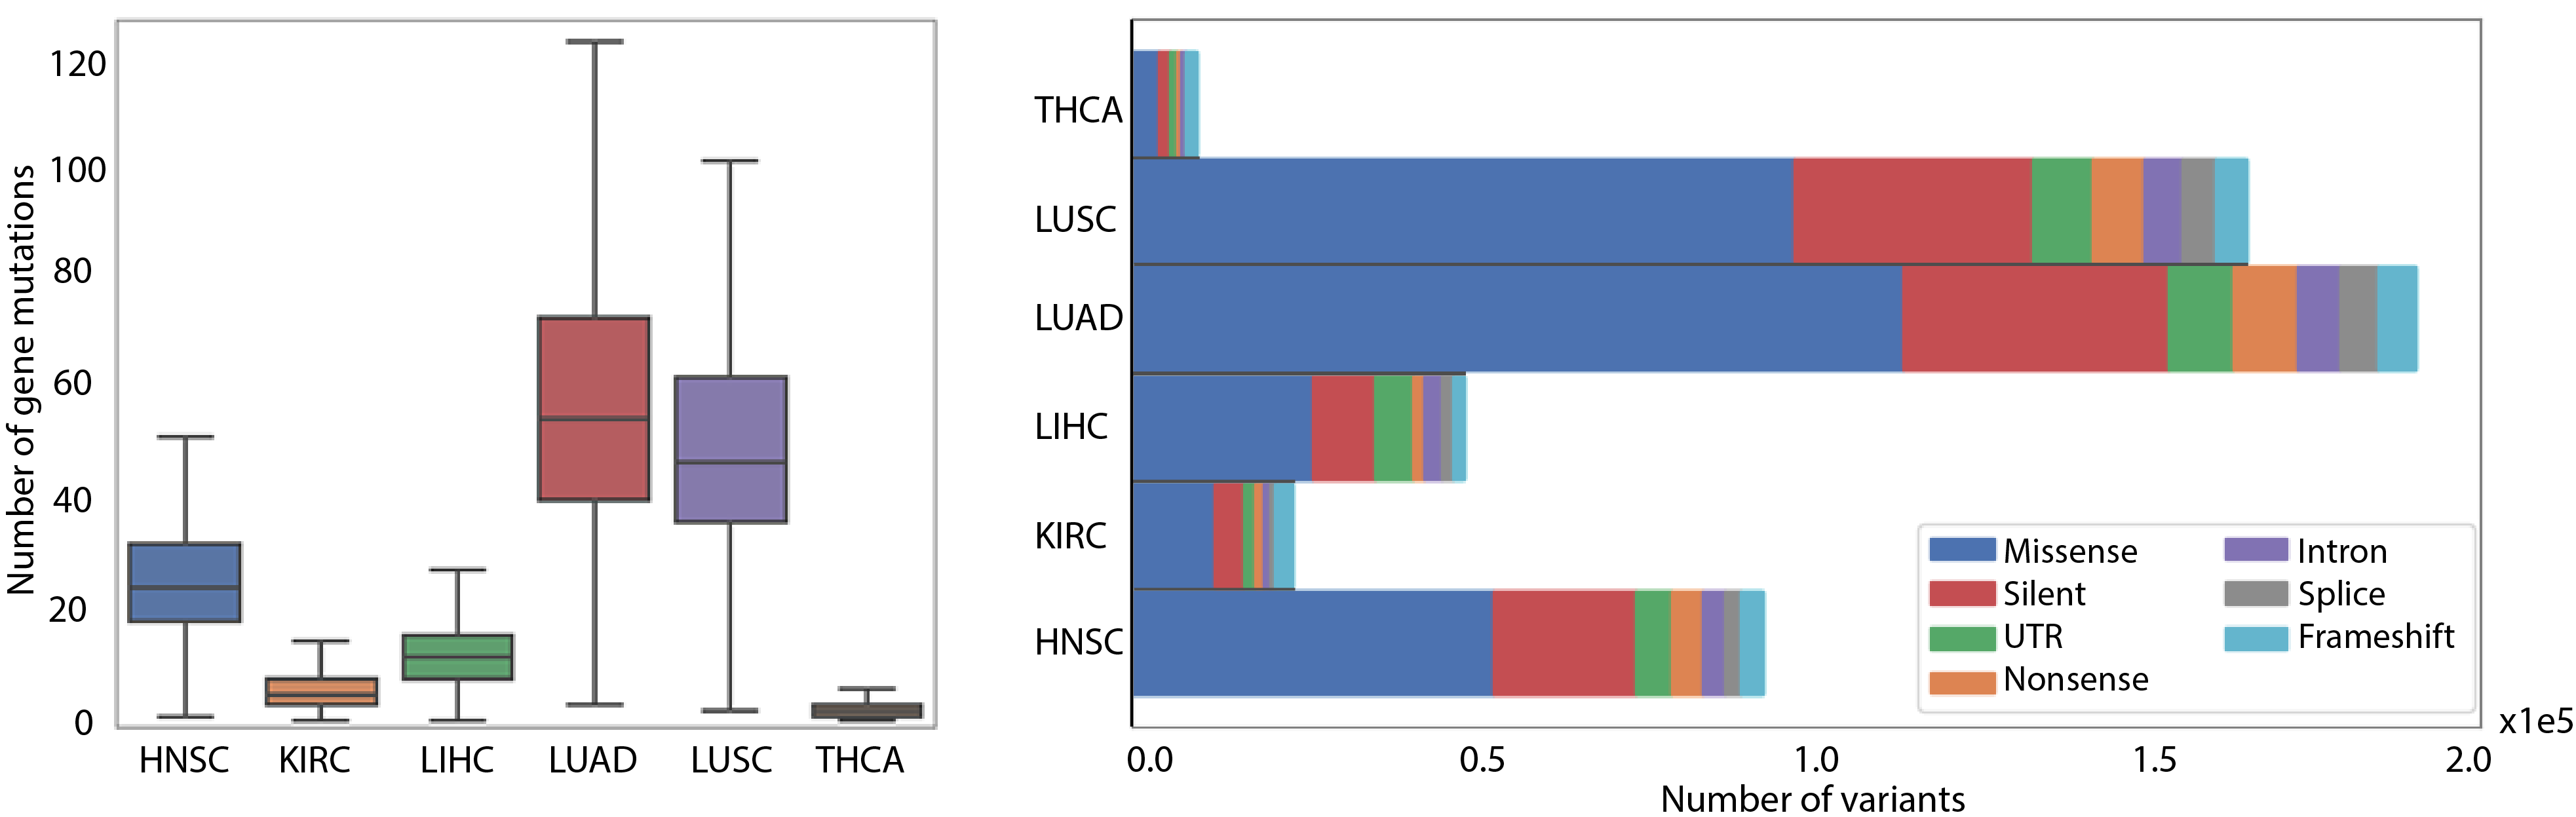
\includegraphics[width=\textwidth]{img/snvstats.png}
    \noindent
    \begin{minipage}[t]{.39\textwidth}
    \raggedright
        a) Accumulated gene mutations
    \end{minipage}% 
    \hspace{1cm}
    \begin{minipage}[t]{.5\textwidth}
        b) Variant classification distribution
    \end{minipage}
    \centering
    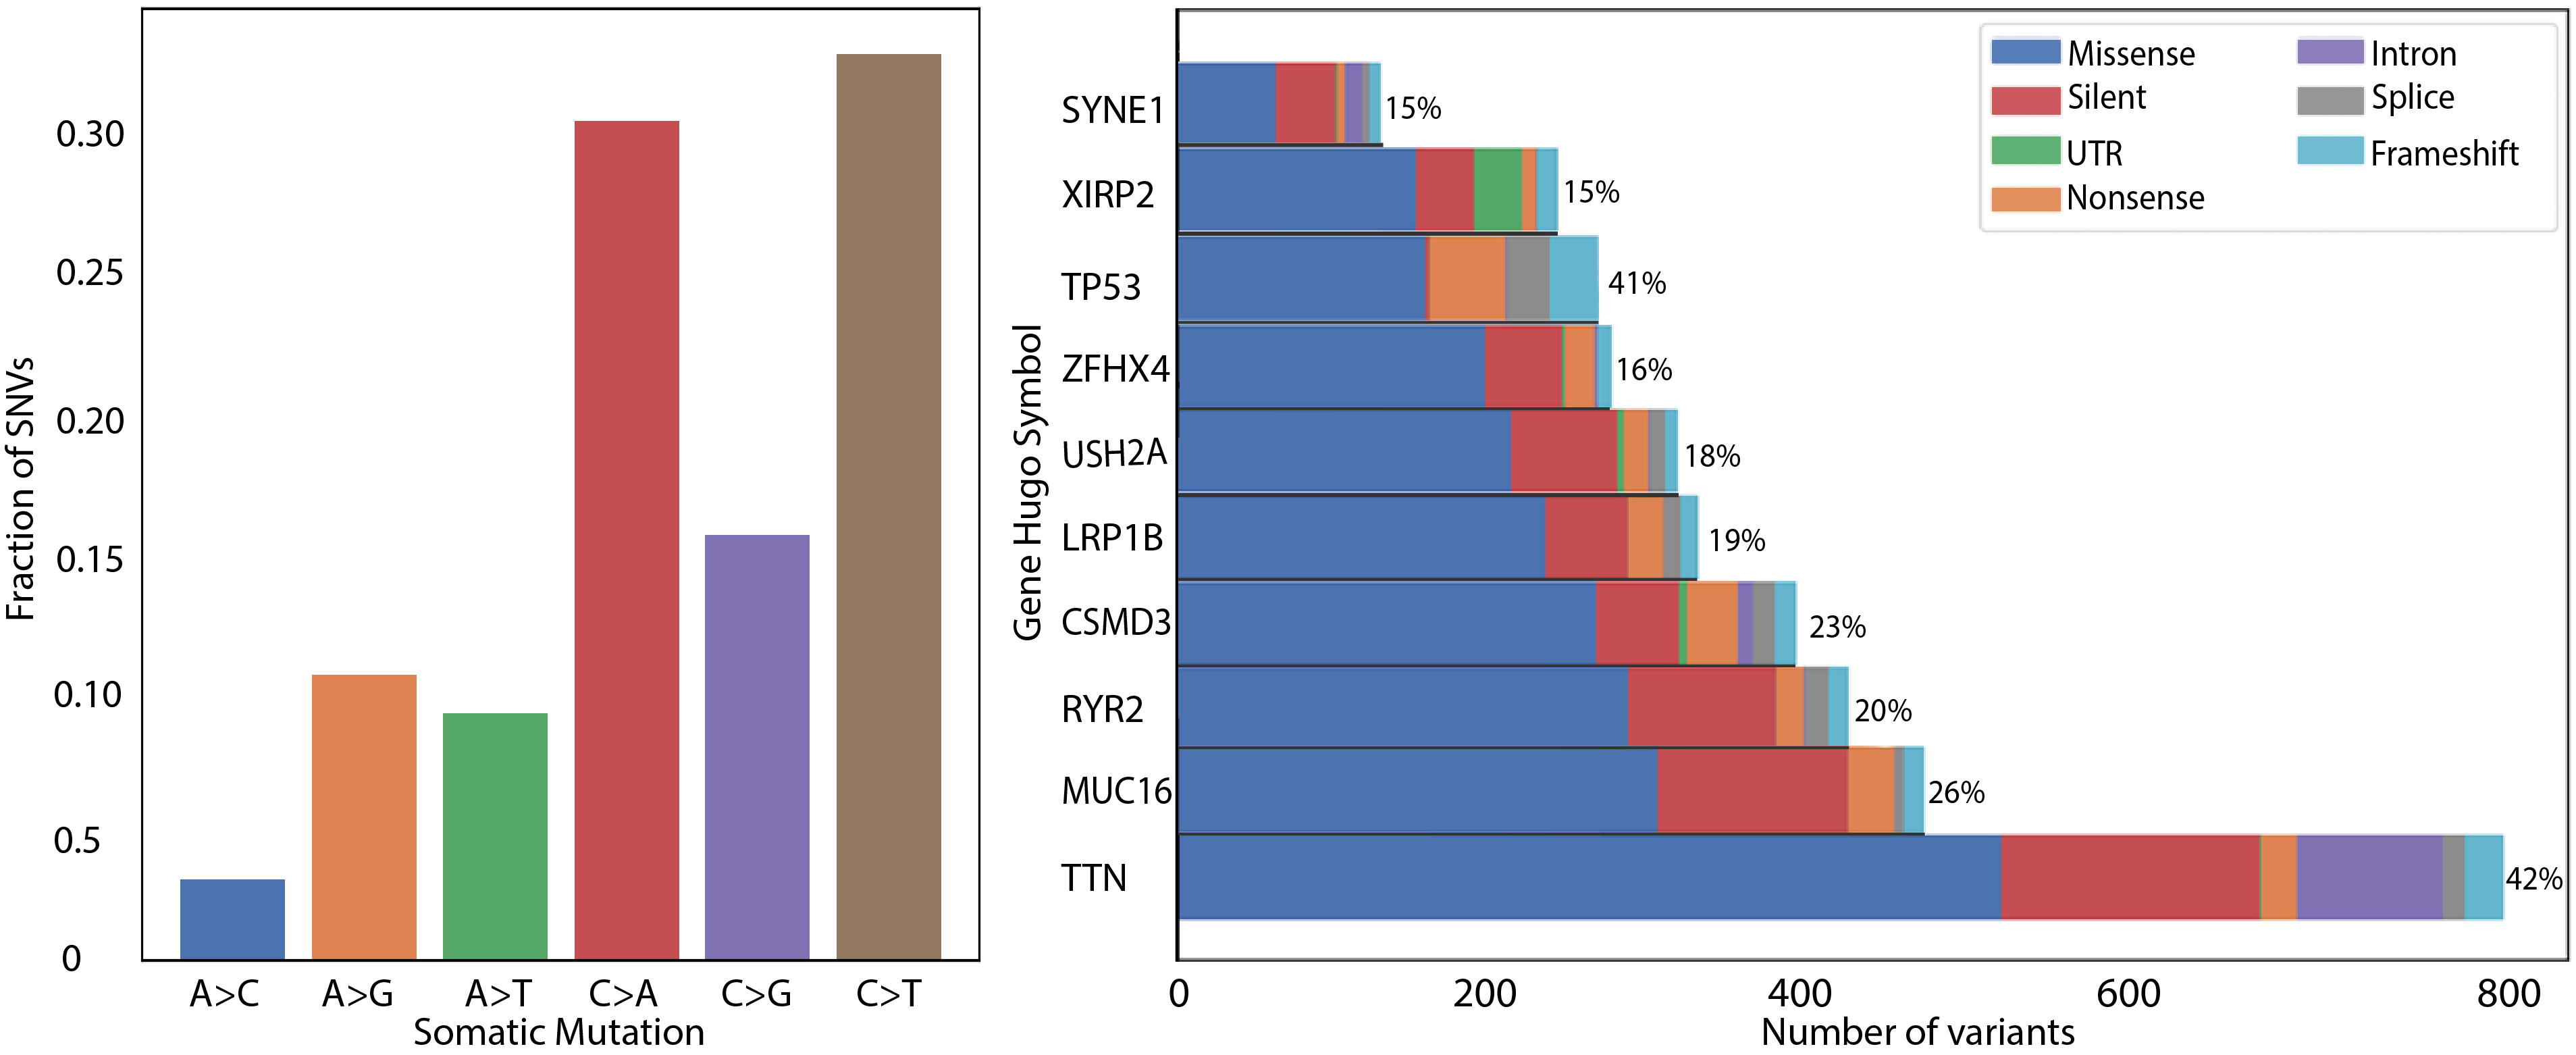
\includegraphics[width=\textwidth]{img/snvstats2.png}
    \noindent
    \begin{minipage}[t]{.39\textwidth}
    \raggedright
        c) Fraction of somatic muations
    \end{minipage}% 
    \hspace{1cm}
    \begin{minipage}[t]{.5\textwidth}
        d) Variant distribution of top 10 mutated genes
    \end{minipage}
    \caption{a) Box plot of accumulated gene mutations for each cancer type. b) Stacked bar plot showing the distribution of variant classification for each cancer type. c) Bar plot showing the fraction of all somatic mutations. d) Stacked bar plot detailing the distribution of the top 10 mutated genes.}
    \label{fig:snvstats}
\end{figure}

In this study, the analysis of the raw SNV data was based on the variant occurrence frequency of the genetic data. Variation occurence was mapped to every listed gene for all available cell samples. This was performed by mapping mutated genes to cell sample IDs in the raw SNV data, and accumulating the number of mutations for each respective cell sample.

\subsubsection{Dataset}

After preprocessing the SNV data, the variant occurrence frequency was obtained for 20516 human genes for each cell mass sample. The variant occurrence frequency was recorded in matrix $S \in \{\mathbb{Z}_{\geq 0}\}^{20516 \; \times \; m}$, where the 20516 rows coorespond to genes, and the m columns correspond to the m cell samples per gene. Accordingly, an entry of the matrix $S$ indicates the number of mutations observed for a cell on a given gene. 

\section{Dimensionality Reduction}

In the following, we describe the various forms of dimensionality reduction used to deal with the high dimensionality of the genomic data and the selection of relevant features. 

\subsection{Stacked Denoising Autoencoder}

%If descriving the model use a present tense, leave the experimental parameters for later

A SDAE was used to acquire compressed feature vectors from all genomic data sources. A two layer SDAE with dimensions 1000, and 500 was trained using a designated training set. Optimal model parameters were selected based on model performance during 10-fold cross validation. Post training, a layer with reduced dimensionality and a low cross validation error was selected. The defined objective here was to acquire a reduced mapping that encodes the original data with minimal loss of meaningful patterns.

%Product of the weight matrix,
%Pliral for the weight matricies
%Multiple the matrcies of the layers 

\subsection{Deeply Connected Genes}

In our experiments, the weights of the trained SDAE were used to extract the raw features most strongly connected to the reduced subspace for CNV, RNA-seq and miRNA-seq data sources. These features were extracted from the SDAE by computing the product of the weight matrices for each layer \cite{danaee2017deep}. 
The product of the weights for each layer in the trained and optimally parametized SDAEs were observed to be highly normally distributed as shown in Fig. \ref{fig:zscoreHist}. 

\begin{figure}[h!]
     \centering
         \centering
         \sidesubfloat[]{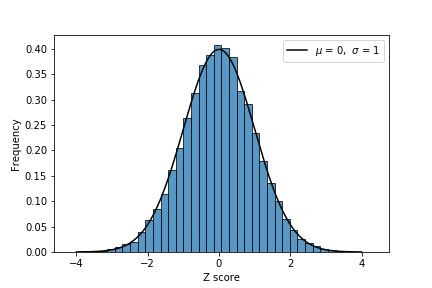
\includegraphics[width=0.25\textwidth]{img/zscoreCNV.png}}
     \hfill
         \centering
         \sidesubfloat[]{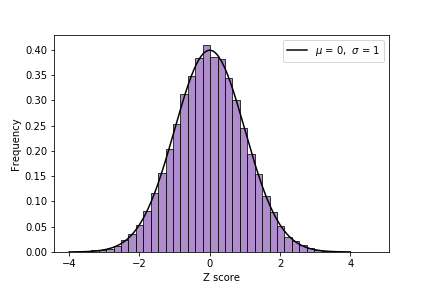
\includegraphics[width=0.25\textwidth]{img/zscoreRNA.png}}
     \hfill
         \centering
         \sidesubfloat[]{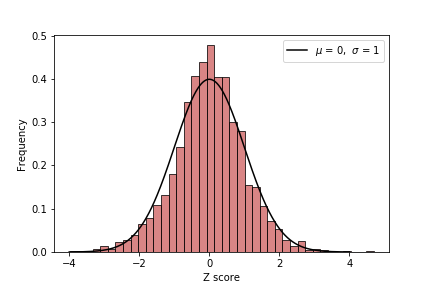
\includegraphics[width=0.25\textwidth]{img/zscoreMIRNA.png}}

        \caption{Histogram of z-scores from dot product of SDAE weight matrices for (a) CNV (b) RNA-seq and (c) miRNA-seq.}
        \label{fig:zscoreHist}
\end{figure}

The most statistically significant features were identified by fitting the weight matrices to a normal distribution, and computing a p value to select features that match the preselected experimental dimensions.

\subsection{Differential Expression}

For the transcriptome expression data, deferentially expressed genes were identified, and utilized as features. The log$_{2}$(fold change) was computed between the median tumour cell mass expression and healthy cell mass expression. The most statistically significant features were identified by fitting the differential expression to a Guassian distribution and computing a two-tailed p-value. Features that match the preselected experimental dimensions were acquired by selecting the top most significant deferentially expressed genes using the two-tailed p-values. 

\begin{figure}[h!]
     \centering
         \centering
         \sidesubfloat[]{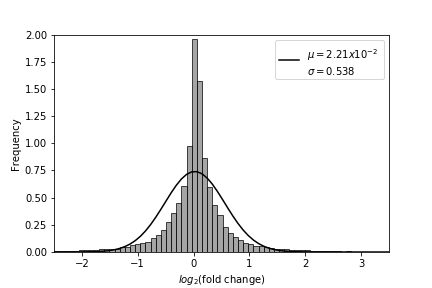
\includegraphics[width=0.4\textwidth]{img/rnaDE.png}}
     \hfill
         \centering
         \sidesubfloat[]{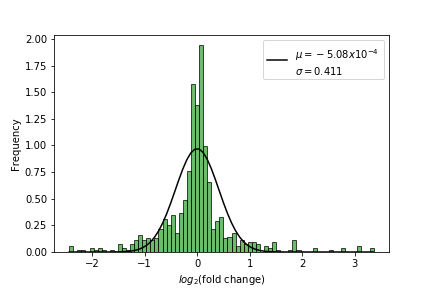
\includegraphics[width=0.4\textwidth]{img/mirnaDE.png}}
        \caption{Differential expression $log_2$(fold change) and Gaussian fit for (a) RNA-seq and (b) miRNA-seq.}
        \label{fig:deHist}
\end{figure}

\subsection{Clustered Gene Filtering}

Due to the sparse nature of the discrete point mutation SNV data, clustered gene filtering (CGF) was used to select a subset of the most discriminatory genes based on the variant occurrence frequency matrix $S$ \cite{yuan2016deepgene}. The procedure involves filtering the genes into groups based on a similarity criteria, and then selecting a subset of genes from each group that have the highest mutation frequency because these are likely of more interest. Dimensionality reduction can be controlled algorithmically through the modulation of distance threshold $d_{cgf}$, and the group element threshold $n_{cgf}$. The distance threshold dictates how similiar the mutation profiles of two genes need to be to be grouped together. The group element threshold is the number of genes kept from each group. The CGF algorithm used is summarized in Algorithm \ref{alg:cgf}.

{\singlespacing
\begin{algorithm}
\caption{Clustered Gene Filtering}\label{alg:cgf}
\begin{algorithmic}[1]
\Require Data matrix $S \in \{\mathbb{Z}_{\geq 0}\}^{p \; \times \; m}$
\Require Distance threshold $d_{cgf} > 0$, and group element threshold $n_{cgf} > 0$
\Procedure{CGF}{$S,d_{cgf},n_{cgf}$}%\Comment{The g.c.d. of a and b}
\State $S_{sum} \gets sum(S, axis=2) $\label{alg:sumA}
\State $S_{sum}^{*} \gets sort(S_{sum}, \textrm{order}=descending)$
\State $S \gets reindex(S, \textrm{index} = S_{sum}^{*})$
\State $g = 0_{1,p}$\label{alg:igsGroup}
\State $\textrm{groupNum} \gets 0$
\For{$i \in \{1 \dotsc p\}$}\label{alg:igsS}
    \If{$g_i = 0$}
        \State $\textrm{groupNum} \gets \textrm{groupNum} + 1$
        \State $g_i = \textrm{groupNum}$
        \For{$j \in \{2 \dotsc p\}$}
            \If{$j \neq i \;\; \textrm{and} \;\; g_{j} = 0$}
                \If{$d(S_{i...},S_{j...}) > d_{cgf}$}
                    \State $g_j = \textrm{groupNum}$
                \EndIf
            \EndIf
        \EndFor    
    \EndIf
\EndFor\label{alg:igsE}
\State $g_{out} \gets \varnothing$\label{alg:igsOut}
\For{$k \in \{1 \dotsc max(g)\}$}
    \For{$\textrm{all} \;\; g_c = k$}
        \If{$g_c > n_{cgf}$}
            \State $g_{out} \gets g_{out} \cup g_{c}[1 \dotsc n_{cgf}]$
        \EndIf
    \EndFor
\EndFor

\State $S_{cgf} \gets S[g_{out},:]$
\State \textbf{return} $S_{cgf}$%\Comment{The gcd is b}
\EndProcedure
\end{algorithmic}
\end{algorithm}}

\noindent
In line \ref{alg:sumA}, we sum matrix $S$ by its second dimension, such that $S_{sum} = \sum_{j} S_{ij}$ is a one dimensional vector of length $p$. We then produce $S_{sum}^{*}$ by sorting matrix $S_{sum}$ in descending order. The matrix $S$ is then reindexed to match the sorted array so that the genes with the highest mutation frequency are listed first. Line \ref{alg:igsGroup} initializes a $p$-dimensional array to store the value of the clustered group for each gene. In steps \ref{alg:igsS} to \ref{alg:igsE}, the genes of matrix $S$ are clustered by inter-gene similarity. The similarity metric between two genes $A$ and $B$ is calculated using the cosine similarity:

\begin{equation}
    d(A,B)= \frac{AB^{T}}{\lVert A \rVert \lVert B \rVert}
\end{equation}

\noindent
In line \ref{alg:igsS}, the index $i$ iterates through the $p$ genes, starting with the gene with the highest mutation frequency $S_1$.  The similarity between this gene and all the remaining genes are calculated, and if the similarity is larger than the threshold $d_{cgf}$, the respective gene is assigned to the group of $S_1$. After the similarity between $S_1$ is computed with all genes, the inter-sample similarity calculations and gene group assignment is repeated for the next ungrouped element in $S$. The last step forms the discriminatory subset by selecting the top $n_{cgf}$ in each group. The indices for the discriminatory subset are stored in the variable $g_{out}$, which is initialized as an empty set in line \ref{alg:igsOut}. The following two for loops iterate through all the genes $g_c$ for a specific group $k$, and stores the top $n_{cgf}$ genes as long as the group does not have fewer then $n_{cgf}$ elements.

\section{Model Interpretation}

%\subsection{Grad-cam}

\subsection{Gene-wise Interpretable Explanations}

To find a gene-wise explanation, the LIME procedure is used to approximate the dGMU model with a linear model of class $G$, such that $g(\tilde{x}) = {w_g}^{T} \tilde{x}$. Perturbed instance $\tilde{x}$ is generated by individually noising each feature by drawing from a normal distribution. The mean and standard deviation is taken from each feature in the original dataset $X$. The perturbed instance is weighted using an exponential kernel learned over a euclidean distance by letting $\mu_{x_i}(\tilde{x}) = exp(-\sqrt{\sum_{i=1}^{n}(x - \tilde{x})^2})/\sigma)$. The kernel width $\sigma$ is defined as 0.75 times the square root of the number of training instances (default value for $\sigma$ is used as established in \cite{ribeiro2016should}). With a locally weighted squared error $J$, as defined in Eq. (\ref{eq:lime}), we learn the weights $w_g$ of the sparse linear model via least squares. Each trained model provides interpretable explanations through the learned weights. The magnitude of a coefficient relates to the importance of the respective gene in sample $x_i$. Furthermore, genes with a positive weight coefficient are positively correlated with the prediction of the dGMU model and genes with a negative weight coefficient are negatively correlated. Accordingly, the explanation of a single prediction provides an interpretable framework by indicating the genes that were most influential. And more specifically, by indicating how the RNA-seq expression or SNV of the gene correlates with the model prediction. 

The gene-wise explanations for a single prediction provides locally faithful insight into the logic of the classifier. In order to assess the global fidelity of the model, gene-wise explanations are pooled to evaluate the reliability of the predictions as a whole. Gene-wise explanations are extended to understand the set of individual instances associated with correctly labelled predictions. Explanations for a set of correctly labelled instances are relevant in understanding the reliability of the classifier and assessing how the model behaves globally. Given the dataset of correctly labelled instances for cancer class $k$, $\mathcal{X}_k$, we construct an $n \times p$ dimensional explanation matrix by setting $\mathcal{W}_{ij} = \xi(\mathcal{X}_k)$. The matrix $\mathcal{W}_{ij}$ represents the local importance of all $n$ genes for each of the $p$ correctly labelled instances for a given class. The gene-wise global weights can then be pooled in an $n$ dimensional vector g = $\sum_{i=1}^{n}\mathcal{W}_{ij}$. Accordingly, genes that explain more instances will be ranked with a higher importance.

